% 第3章 視覚的顕著性
\newpage
\renewcommand{\baselinestretch}{1.5}
\section{視覚的顕著性}\label{sec:visula_saliency}
\renewcommand{\baselinestretch}{1}
\par 本章では、本研究を説明する上で最も大切なキーワードである視覚的顕著性やそれらを可視化する視覚的顕著性マップについて説明する。

\subsection{視覚的顕著性とは}
\par 我々の注意や注目は視覚的に顕著な刺激に引き付けられる。視覚的顕著性とは人の注視の引き付けやすさを示す指標で、空間的配置の関係によりボトムアップの視覚刺激を引く起こす特性のことを言う。また、周囲と比較して目立つことを顕著性が高いと表現する。図\ref{fig_whats-saliency}に視覚的顕著性の例を示す。左図の例を見てみると一つだけ赤色の棒が存在し周りの緑色の棒と比較すると目立って見える。また、真ん中の例を見ると全て色が同じだが一つだけ方向が異なる棒が存在し目立って見えると思う。最後に右図の例を見ると、一つだけ垂直方向に向いている赤い棒があるがほとんど分からない。このように特定の要素を周りの要素の位置やコントラストや方向などの特性から際立たせる事で注意を引かせるようにする主観的な知覚品質の事を示す\cite{Itti:2007}。

\begin{figure}[H]
    \centering
    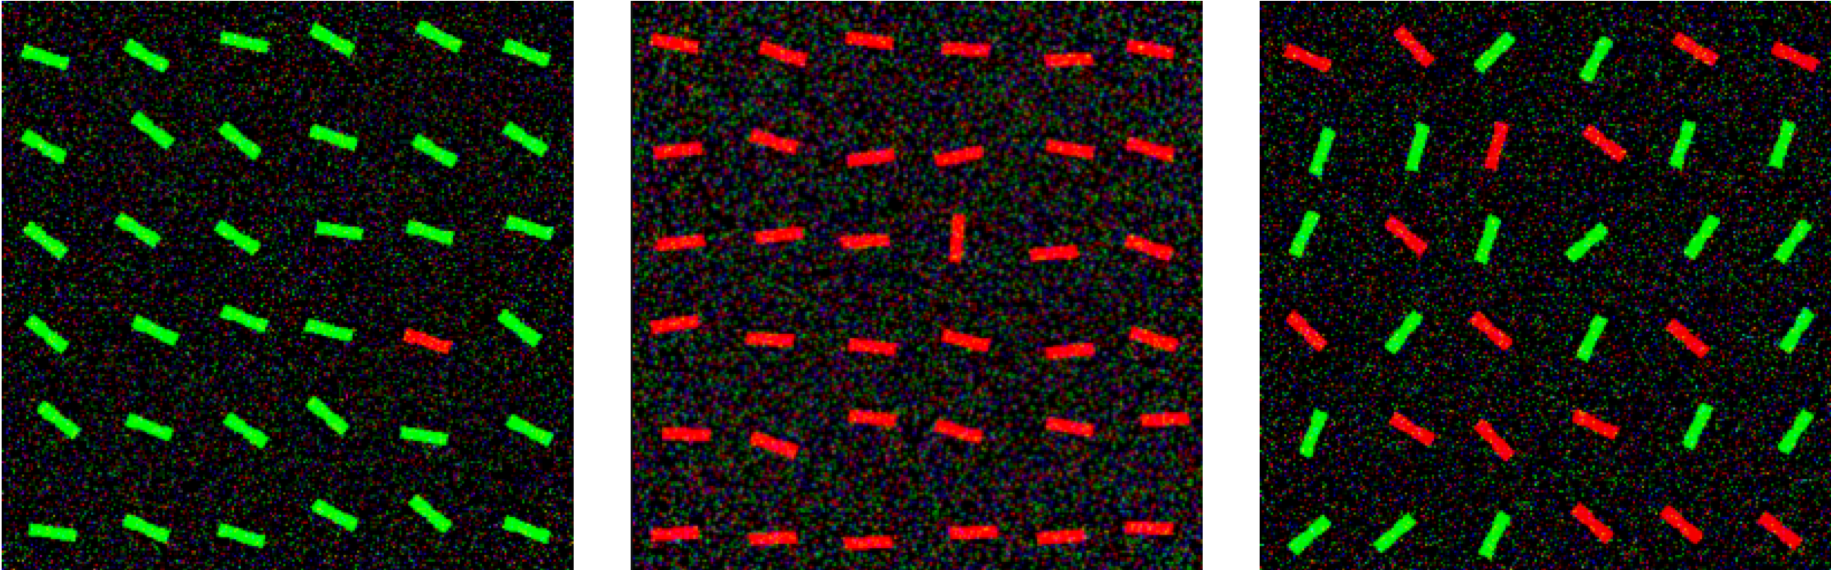
\includegraphics[width=12cm]{figures/whats-saliency.png}
    \caption{視覚的顕著性の例\cite{Itti:2007}}
    \label{fig_whats-saliency}
\end{figure}

\subsection{視覚的顕著性マップ}\label{subsec:saliency_map}
\par 色や輝度や方向などの視覚の基本的な特徴マップを足し合わせることにより解析対象の画像から各ピクセルの注視の度合いである顕著性を推定して作成したヒートマップを視覚的顕著性マップという。図\ref{fig_03_ex-saliencymap}に自然画像である桜の画像を入力した時に生成される視覚的顕著性マップの例を示す。顕著性マップには大きく分けてグレースケール形式とヒートマップ形式の2種類がある。グレースケール形式の視覚的顕著性マップは白から黒までの明暗で表現するグレースケールで描写され、明るい領域が顕著性が高く注目されやすい領域で、逆に暗い領域は顕著性が低く注目されにくい領域であるという事を表す。ヒートマップ形式の視覚的顕著性マップは色の濃淡で顕著性を描写され、暖色になればなるほど顕著性が高く逆に寒色になればなるほど顕著性が低くなることを表す。これらの顕著性が高い領域を可視化した視覚的顕著性マップを見ることとでユーザーがどの領域に注目する可能性が高いのかを認識することが可能となる。

\begin{figure}[H]
    \centering
    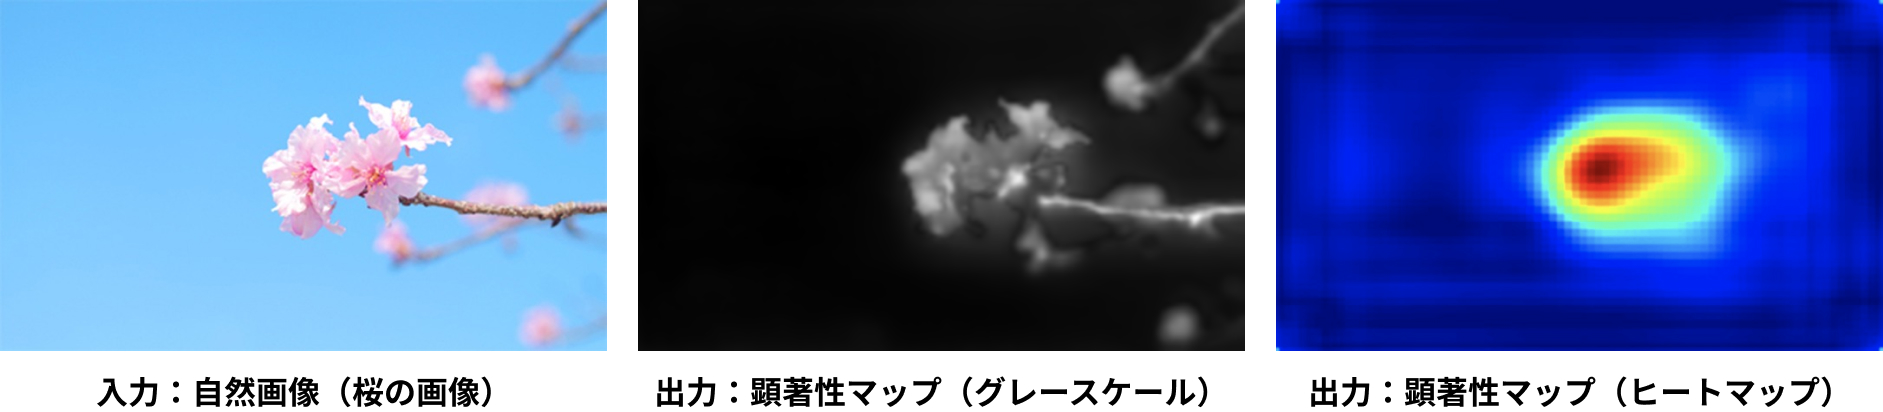
\includegraphics[width=12cm]{figures/03_ex-saliencymap.jpg}
    \caption{顕著性マップの出力例}
    \label{fig_03_ex-saliencymap}
\end{figure}

\subsection{顕著性マップ生成モデル}
\par 第\ref{subsec:saliency_map}節で説明した視覚的顕著性マップを生成するモデルのことを顕著性マップ生成モデルという。多くのモデルは人間の目と同じように位置特性、方向特性、輝度特性などのボトムアップ要因を組み合わせて顕著性マップの生成を行う。また近年機械学習や深層学習の技術が進みニューラルネットワークを使用したモデルも多数研究されている。しかしながら、それらの研究のほとんどは街並みや風景などの自然画像の顕著性マップ生成モデルに関するもので、ウェブページに特化した顕著性マップの生成モデルについての研究はほとんど存在しない。自然画像と比較するとウェブページにはテキスト、写真、ロゴ、アニメーションなどのウェブページ固有の独特な特徴が存在する為、これらが正確な顕著性の予想を困難にする。